\section{Überarbeitung der Dongle-App}
Die Dongle-App dient neben dem nrf\_Base Projekt als Basis für die Anwendung des Fußschalters. Sie diente als Proof-of-Concept und ermöglichte als solche die Bereitschaft des Projektmanagements die Ressourcen für die Implementierung des Fußschalters zu bewilligen. Im ersten Schritt der Implementierung wird sie um Grundfunktionalitäten erweitert und die Datenverarbeitung fehlertoleranter gestaltet.

\subsection{Trennung der Projekte}
Das Framework der Hoffmann Group zur Abstraktion der \ac{BLE}-Schnittstelle nrf\_Base wird in allen \ac{HCT}-fähigen Produkten eingesetzt und stetig weiterentwickelt. Um die fehlerfreie Kommunikation des Fußschalters zu den \ac{HCT}-Werkzeugen auch in Zukunft sicherzustellen, müssen Updates des nrf\_Base auch in das Projekt des Fußschalters übernommen werden. Während in der Proof-of-Concept Anwendung des Dongles darauf noch keine Rücksicht genommen wurden, soll in der Entwicklung des Fußschalters von Anfang an diese Abhängigkeit berücksichtigt werden und die Dongle-App entsprechend angepasst werden. Des weiteren soll auch der Umfang der Anwendung, die auf dem Dongle läuft, minimiert werden und der Code für die Peripherie des Fußschalters abgetrennt werden. Wiederum in anderen Produkten als dem Dongle und dem Fußschalter, darf deren Code nicht zu finden sein.

Folgende Peripherie darf dabei nur in den jeweiligen Projekten initialisiert werden:
\begin{itemize}
	\item nrf\_Base: UART
	\item \ac{HCT}-FootSwitch: Fußschalter, Akku Power Management, Drei-Farben LED, \ac{USB}
	\item Dongle: Ein-Farben LED, \ac{USB}
\end{itemize}

Um diese Anforderungen zu erfüllen kann einerseits für alle drei Projekte eine eigene Codebasis geschaffen werden, die sich jeweils stark überschneiden und gesondert gepflegt werden müssen oder die selbe Codebasis für alle Projekte benutzt werden. Die erste Möglichkeit hat den Vorteil, dass sich die Entwicklung einfacher gestaltet, da auf diese Abhängigkeiten keine Rücksicht genommen werden muss. Zudem kann der Code stärker auf den Anwendungsfall optimiert werden, jedoch macht der enorme Arbeitsaufwand die gesonderten Codebasen zu unterhalten und auf dem neuesten Stand zu halten, diese Möglichkeit unpraktikabel. Des weiteren wurde aus Software architektonischen Gründen die Anwendung bereits gekapselt, wodurch die programmatische Abtrennung der Teile keinen außerordentlichen Entwicklungsaufwand erfordert.\\
Stattdessen muss aus der Main-Routine nur zwei Funktionsaufrufe mit Compilerschaltern abgetrennt werden, um den Code des Fußschalter bzw. Dongles vom nrf\_Base Projekt zu trennen. Zum einen der Initialisierungsaufruf und ein App-process Aufruf, da der Main-Loop als Dispatcher für die gesamte Anwendung fungiert. Im Central müssen die Datencallbacks, sowie im Connection State Callback die Aufrufe an die Dongle-App abgetrennt werden. Die Funktionalität der UART stellte sich als wenig gekapselt heraus und musste an zahlreiche Stellen kleinteilig aus dem Fußschalterprojekt abgetrennt werden.\\ 
Das ambitioniertes Ziel war dabei, dass nach der Einführung der Compilerschalter das Binärfile des nrf\_Base Projekts identisch zu der vorangegangenen Version ohne Fußschalter sein sollte. Aus noch nicht geklärten Umständen ist das jedoch nicht der Fall.


\subsection{Verbesserung Verbindungsaufbau}
Im ersten Prototyp der Dongle-App wird nach dem Einlesen der Konfigurationsdatei, überprüft ob die jeweiligen Geräte bereits verbunden sind. Falls ein Gerät unverbunden ist, wird das Scanning gestartet und periodisch die vom Central gefundenen Geräte auf das zu verbindende Gerät hin überprüft. Ist es schließlich gefunden, wird der Verbindungsaufbau angestoßen und sobald die Service discovery vollzogen wurde, wird sich auf die \ac{BLE}-\ac{HCT}-Charakteristik subscribed und das Connection Handle des Geräts aus dem Central Device übernommen. \\
Dabei werden jedoch zwei Zustände nicht abgebildet. Zum einen wird zwischen der Verbindungsaufnahme und der Subscription auf die \ac{BLE}-\ac{HCT}-Charakteristik, der Zustand ``Connected'' eingenommen. Hier wird bereits das Connection Handle zugeordnet und muss gespeichert werden, da ab der Einnahme dieses Zustands ein Verbindungsabbruch auftreten und nur über das Connection Handle nachvollzogen werden kann. Zum anderen wird nach der erfolgreichen Subscription ein Acknowledgement übermittelt und im Central der Zustand ``Subscription'' eigenommen. Hier wurde in der Dongle-App bereits das Connection Handle dem Gerät zugeordnet, weswegen ein Disconnect nachvollzogen werden kann, jedoch wird die initiale Kommunikation mit der Abfrage der Messeinheit forgesetzt. Dabei wurde bisher nicht gewartet, dass die Subscription erfolgreich abgeschlossen wurde, was jedoch die Zuverlässigkeit des Verbindungsaufbaus und der Abfrage der Messeinheit erhöht.\\
Dabei wurde die Callback Funktion bisher direkt im Eventhandler des Central aufgerufen. Diese Erweiterung hätte es erfordert, eine respektiven Callback in allen zugehörigen Events aufzurufen, was entgegen der Kapselung der Projekte geht. Jedoch gibt es im Central bereits eine ähnliche Funktionalität, die den Zustand des Central Moduls über UART ausgibt und bereits in den Events des Verbindungsaufbaus aufgerufen wird. Sie wird nun erweitert, sodass falls der Compilerschalter für die \ac{USB}-App gesetzt ist, der Zustand des Moduls nicht über UART, sondern an einen Callback der \ac{USB}-App überreicht wird. In der \ac{USB}-App wird der Zustand gespeichert und die dazugehörigen Folgeaktionen durchgeführt. Im Central Modul ist weiterhin nur ein einziger Aufruf einer \ac{USB}-App Funktion vonnöten, um die Zustände des Verbindungsaufbaus in der \ac{USB}-App abzubilden.

\begin{figure}[H] 
	\centering
	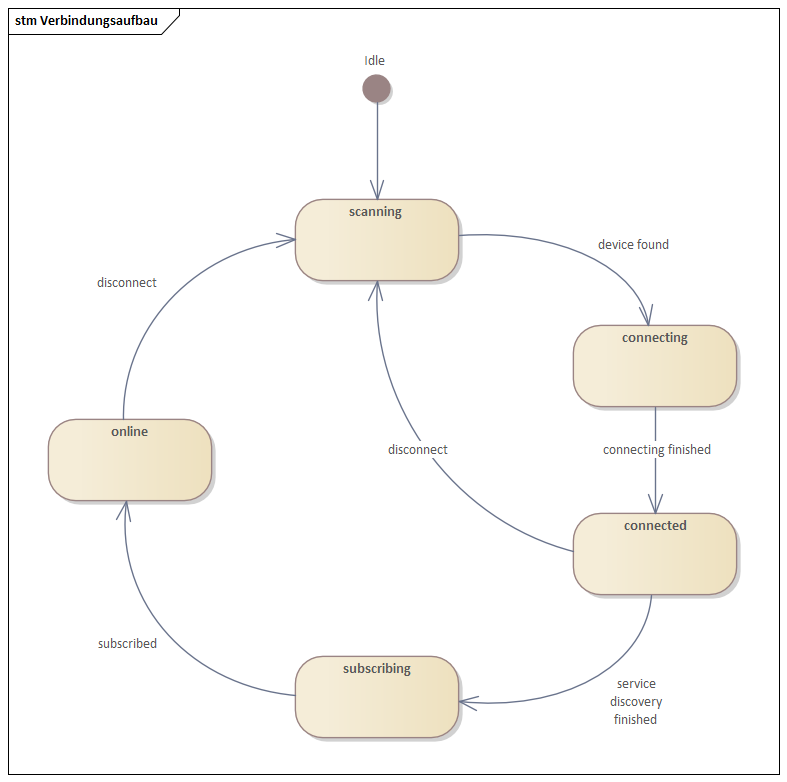
\includegraphics[width=\textwidth]{figures/Verbindungsaufbau.png}
	\caption{Zustandsdiagramm des Verbindungsaufbaus}
\end{figure}



\subsection{Optimierung Abfrage Messeinheit} 
Im Ausgangszustand der \ac{USB}-Dongle App muss die Anwendung bei Werkzeug der Marke Holex jedes Mal, wenn sie ein Messergebnis erhält, die Einheit der Messung abfragen. Bei Drehmomentschlüsseln der Marke Garant wird ein Datenblock mit der Messeinheit kurz nach Erhalten des Messergebnisses empfangen. Diese Nachricht bezieht sich jedoch auf die derzeitig eingestellte Messeinheit, welche im Fall eines Arbeitsablaufs mit sich ändernden Einheiten, die Einheit für die nächste Messung ist. In diesem Fall gibt die \ac{USB}-Dongle App die falsche Einheit aus. Bei Geräten der Marke Holex wird nur bei einer Änderung der Messkonfiguration, diese übermittelt.\\
In beiden Fällen sendet das Werkzeug automatisch bei einer Änderung der Messkonfiguration einen Datenblock mit der Messeinheit an die Subscriber der \ac{HCT}-Charakteristik. Die Kontrolle der Messeinheit kann daher verbessert werden, indem die derzeitig eingestellte Messeinheit nach dem Verbindungsaufbau einmal abgefragt wird und für jedes verbundene Gerät gespeichert wird. Bei einer Änderung der Messeinheit wird die Dongle-App notifiziert und die gespeicherte Einheit aktualisiert. Dadurch wird eine fehlerhafte Einheit in der Ausgabe vermieden und die Anzahl an Nachrichten der Dongle-App an das Messgerät verringert.

\begin{figure}[H] 
	\centering
	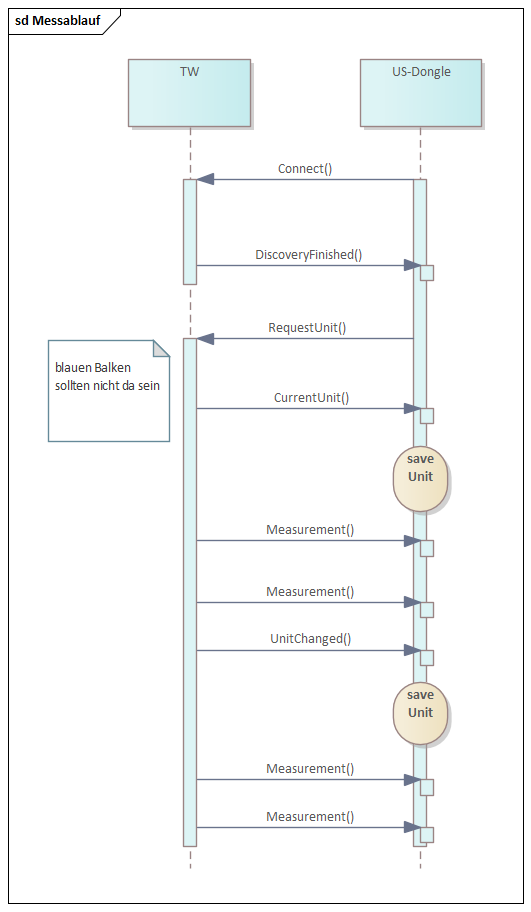
\includegraphics[width=\textwidth]{figures/Messablauf.png}
	\caption{Messablauf}
\end{figure}

